\documentclass[main.tex]{subfiles}
\pagenumbering{arabic}
\newcommand\chapterlabel{ChMIX-biomoleculesinsolution}\setcounter{figurenewcounter}{0}\setcounter{tablenewcounter}{0}\setcounter{formulanewcounter}{0}
\setcounter{chapter}{2}

\begin{document}



\chapter[Gases  ]{Gases }

\begin{marginfigure}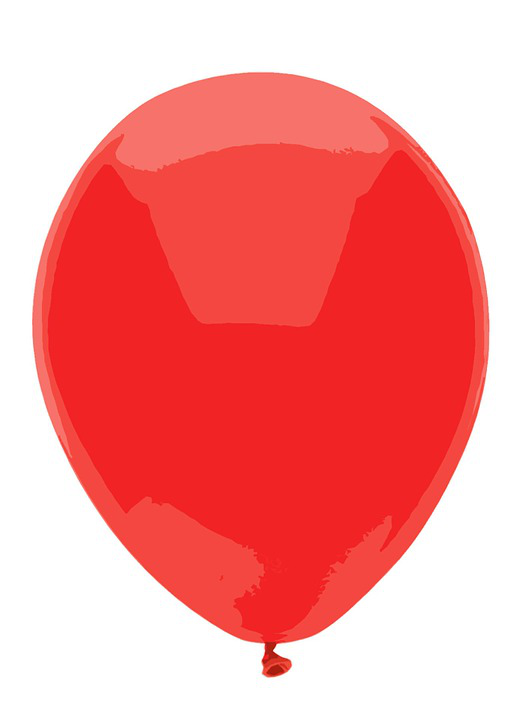
\includegraphics{../Ch-Gas/figure1} \end{marginfigure}\import{../Ch-gas/files/}{ChapterIntro}

\begin{marginfigure}%LEARNING GOALS BOX
\begin{mytcbox}{GOALS}
%
\begin{center}\textcolor{blue}{\faEnvira Chemistry and molecules }\end{center}
%\begin{enumerate}[label=\protect\circled{\color{white}\arabic*}]
%%  \import{../Ch-Gas/files/}{SectionGoal-Simple-Carbohydrates}
%% \import{../Ch-Gas/files/}{SectionGoal-Disaccharides-and-polysaccharides}
%\end{enumerate}

\begin{center}\textcolor{blue}{\faFlask Acids and bases }\end{center}
%\begin{enumerate}[label=\protect\circled{\color{white}\arabic*}]
%%\import{../Ch-naming/files/}{SectionGoal-Ionic-compounds}
%%\import{../Ch-naming/files/}{SectionGoal-Naming-acids-bases}
%\end{enumerate}

\begin{center}\textcolor{blue}{\faTint  Electrolytes and solutions }\end{center}
%\begin{enumerate}[label=\protect\circled{\color{white}\arabic*}]
%%\import{../Ch-electrolytes/files/}{SectionGoal-Electrolytes-and-insoluble-compounds}
%%\import{../Ch-naming/files/}{SectionGoal-Naming-complex-salts-common-chemicals}
%\end{enumerate}

\begin{center}\textcolor{blue}{\faFire Reactions and energy} \end{center}
\begin{enumerate}[label=\protect\circled{\color{white}\arabic*}]
 \import{../Ch-mole/files/}{SectionGoal-Chemical-reaction-Balancing-chemical-reactions}
\end{enumerate}

\begin{center}\textcolor{blue}{\faFlash The chemistry of cancer} \end{center}
%\begin{enumerate}[label=\protect\circled{\color{white}\arabic*}]
%%\import{../Ch-nuclear/files/}{SectionGoal-Radiation-protection}
%	\end{enumerate}
	
\begin{center}\textcolor{blue}{\faFlash Let's calculate} \end{center}
\begin{enumerate}[label=\protect\circled{\color{white}\arabic*}]
\import{../Ch-measurements/files/}{SectionGoal-Using-Conversion-Factors}
\end{enumerate}
			 				 




\end{mytcbox}
\vspace{1cm}
%\begin{tcolorbox}[enhanced,colback=red!5!white,colframe=black!50!red,boxrule=1pt,
%  arc=0pt,outer arc=0pt,drop heavy lifted shadow]
%\faGears\ 
% \import{../Ch-electrolytes/files/}{ChapterDiscussion}
% \end{tcolorbox}
\end{marginfigure}%LEARNING GOALS BOX






\renewcommand\chapterlabel{Ch-Gas}



\section{\faEnvira Gases and its properties} \import{../\chapterlabel/files/}{SectionIntro-Gases-and-its-properties}
\sloppy \begin{description}
\item[\docfilehook{Gases in the periodic table}{}]  \import{../\chapterlabel/files/}{SubSection-Gases-and-its-properties-Gases-in-the-periodic-table}
\item[\docfilehook{Characteristics of gases}{}]  \import{../\chapterlabel/files/}{SubSection-Gases-and-its-properties-Characteristics-of-gases}
 \item[\docfilehook{Volume, V}{}] \import{../\chapterlabel/files/}{SubSection-Gases-and-its-properties-Volume,-V}
 \item[\docfilehook{Temperature, T}{}]\import{../\chapterlabel/files/}{SubSection-Gases-and-its-properties-Temperature,-T}
 \import{../\chapterlabel/files/}{Figure-Gas-Table}
 \item[\docfilehook{Amount of gas, n}{}] \import{../\chapterlabel/files/}{SubSection-Gases-and-its-properties-Amount-of-gas,-n}
 \import{../\chapterlabel/files/}{SideFigure-Gases}
\item[\docfilehook{Pressure, P}{}] \import{../\chapterlabel/files/}{SubSection-Gases-and-its-properties-Pressure,-P}
\import{../\chapterlabel/problems/}{SampleProblem1}
 \import{../\chapterlabel/files/}{Figure-Pressure}
\end{description}




 \section{\faEnvira Ideal gas law}\import{../\chapterlabel/files/}{SectionIntro-Ideal-gas-law}
\sloppy \begin{description}
 \import{../\chapterlabel/files/}{SubSection-Ideal-gas-law-Ideal-gas-law-in-terms-of-moles}
\import{../\chapterlabel/problems/}{SampleProblem2}
 \import{../\chapterlabel/files/}{SubSection-Ideal-gas-law-Ideal-gas-law-in-terms-of-density}
\import{../\chapterlabel/problems/}{SampleProblem3}
 \import{../\chapterlabel/files/}{SubSection-Ideal-gas-law-STP-conditions}
\import{../\chapterlabel/problems/}{SampleProblem4}
\end{description}


 \section{\faEnvira Change of gas properties}\import{../\chapterlabel/files/}{SectionIntro-Change-of-gas-properties}
\sloppy \begin{description}
\item[\docfilehook{Solving problems with an initial and final state}{}]  \import{../\chapterlabel/files/}{SubSection-Change-of-gas-properties-Solving-problems-with-an-initial-and-final-state}
\import{../\chapterlabel/problems/}{SampleProblem5}
\item[\docfilehook{Pressure-Volume change}{}] \import{../\chapterlabel/files/}{SubSection-Change-of-gas-properties-Pressure-Volume-change}
 \item[\docfilehook{Volume-Moles change}{}] \import{../\chapterlabel/files/}{SubSection-Change-of-gas-properties-Volume-Moles-change}
\item[\docfilehook{Relating the different variables of a gas}{}]  \import{../\chapterlabel/files/}{SubSection-Change-of-gas-properties-Relating-the-different-variables-of-a-gas}
\end{description}



%  \section{\faEnvira Kinetic molecular theory of gases }\import{../\chapterlabel/files/}{SectionIntro-the-kinetic-molecular-theory-of-gases}
% \sloppy 
%\begin{description}
% \item[\docfilehook{Kinetic theory of gases}{}] \import{../\chapterlabel/files/}{SubSection-Real-gases-and-the-kinetic-molecular-theory-of-gases-Kinetic-theory-of-gases}
%\import{../\chapterlabel/problems/}{SampleProblem11}
%\end{description}
 



 
 \section{\faTint Mixtures of gases  }\import{../\chapterlabel/files/}{SectionIntro-Mixtures-of-gases-and-gas-stoichiometry}
\sloppy 
\begin{description}
 \item[\docfilehook{Partial and total pressure}{}] 
\import{../\chapterlabel/files/}{SubSection-Mixtures-of-gases-and-gas-stoichiometry-Partial-and-total-pressure}
\import{../\chapterlabel/problems/}{SampleProblem7}
 \import{../\chapterlabel/files/}{Figure-Partial-Pressure}
\item[\docfilehook{Partial pressure of a gas in a mixture}{ }]  \import{../\chapterlabel/files/}{SubSection-Mixtures-of-gases-and-gas-stoichiometry-Partial-pressure-of-a-gas-in-a-mixture}
\item[\docfilehook{Mole fraction}{}]  \import{../\chapterlabel/files/}{SubSection-Mixtures-of-gases-and-gas-stoichiometry-Mole-fraction}
\import{../\chapterlabel/problems/}{SampleProblem8}
\end{description}





 



\renewcommand\chapterlabel{Ch-naming}
\section{\faEnvira Covalent compounds}
\import{../\chapterlabel/files/}{SectionIntro-Covalent-compounds}
\sloppy \begin{description}
\import{../\chapterlabel/files/}{Subsection-Covalent-compounds-Covalent-naming}
 \import{../\chapterlabel/files/}{Table-Covalent-prefixes}	
\import{../\chapterlabel/problems/}{SampleProblem5}
\import{../\chapterlabel/files/}{Subsection-Covalent-compounds-Properties-of-covalent-compounds}
\import{../\chapterlabel/files/}{Subsection-Covalent-compounds-The-covalent-bond}
\end{description}



\renewcommand\chapterlabel{Ch-nuclear}
\section{\faFlash Radioactive gases: radon}
\import{../\chapterlabel/files/}{SectionIntro-Radioactive-gases:-radon}

\renewcommand\chapterlabel{Ch-acidbase}

\section{\color{blue!30!black}{\faFlask Blood as a buffer}}\import{../\chapterlabel/files/}{SectionIntro-Blood-as-a-buffer}
\sloppy
\begin{description}
\item[\docfilehook{ Carbon dioxide is an acid}{}] \import{../\chapterlabel/files/}{SubSection-Blood-as-a-buffer-Carbon-dioxide-is-an-acid}
\item[\docfilehook{ The dangerous change in blood PH}{}] 
\import{../\chapterlabel/files/}{SubSection-Blood-as-a-buffer-The-dangerous-change-in-blood-PH}
  \import{../\chapterlabel/files/}{Figure-Alkalosis-and-PH}
\item[\docfilehook{ Alkalosis and carbon dioxide}{}] 
\import{../\chapterlabel/files/}{SubSection-Blood-as-a-buffer-Alkalosis-and-carbon-dioxide}
   \import{../\chapterlabel/problems/}{SampleProblem20}
 \end{description}

\renewcommand\chapterlabel{Ch-mole}
\section{\faFire Chemical reactions}
\import{../\chapterlabel/files/}{SectionIntro-Chemical-reaction}
\sloppy\begin{description}
\import{../\chapterlabel/files/}{SubSection-Chemical-reaction-Simple-chemical-reactions}
\import{../\chapterlabel/files/}{SubSection-Chemical-reaction-Reading-a-chemical-reaction}
\import{../\chapterlabel/files/}{SubSection-Chemical-reaction-Balanced-chemical-reactions}
\import{../\chapterlabel/problems/}{SampleProblem5}
\end{description}

\renewcommand\chapterlabel{Ch-measurements}
\section{\faGears Using Conversion Factors}
\sloppy\begin{description}
\item[\docfilehook{Square or cubic units}{}]\import{../\chapterlabel/files/}{SubSection-Using-Conversion-Factors-Square-or-cubic-units}
\import{../\chapterlabel/problems/}{SampleProblem5}
\item[\docfilehook{Units of volume}{}]\import{../\chapterlabel/files/}{SubSection-Using-Conversion-Factors-Units-of-volume}
\import{../\chapterlabel/problems/}{SampleProblem6}
\end{description}

%\section{ \faEnvira Simple Carbohydrates}
%\import{../Ch-biochemistry/files/}{SectionIntro-Simple-Carbohydrates}
%\sloppy\begin{description}
%\newpage
%\item[\docfilehook{Carbs are made of C, H and O}{}] \import{../Ch-biochemistry/files/}{SubSection--Simple-Carbohydrates-Carbs-are-made-of-C-H-and-O}
%\item[\docfilehook{Monosaccharides: aldo or keto?}{}] \import{../Ch-biochemistry/files/}{SubSection--Simple-Carbohydrates-Monosaccharides-aldo-or-keto}
%  \import{../Ch-biochemistry/problems/}{SampleProblem1}
%\item[\docfilehook{Some important monosaccharides}{}] \import{../Ch-biochemistry/files/}{SubSection--Simple-Carbohydrates-Some-important-monosaccharides}
%\item[\docfilehook{$d-$ and $l-$ monosaccharides}{}] \import{../Ch-biochemistry/files/}{SubSection--Simple-Carbohydrates-d-and-l-monosaccharides}
%\import{../Ch-biochemistry/problems/}{SampleProblem2}
%\item[\docfilehook{Skeletal structure of  monosaccharides}{}] \import{../Ch-biochemistry/files/}{SubSection--Simple-Carbohydrates-Skeletal-structure-of--monosaccharides}
%\item[\docfilehook{Haworth cyclic structure of  monosaccharides}{}] \import{../Ch-biochemistry/files/}{SubSection--Simple-Carbohydrates-Haworth-cyclic-structure-of--monosaccharides}
%\item[\docfilehook{$\alpha$ or $\beta$ form of Cyclic monosaccharides}{}] \import{../Ch-biochemistry/files/}{SubSection--Simple-Carbohydrates-alpha-or-beta-form-of-Cyclic-monosaccharides}
%\import{../Ch-biochemistry/problems/}{SampleProblem3}
%\item[\docfilehook{Obtaining Haworth cyclic structure of monosaccharides}{}] \import{../Ch-biochemistry/files/}{SubSection--Simple-Carbohydrates-Obtaining-Haworth-cyclic-structure-of-monosaccharides}
%\end{description}
%
%
%\section{ \faEnvira Disaccharides and polysaccharides}
%  \import{../Ch-biochemistry/files/}{SectionIntro-Disaccharides-and-polysaccharides}
%\sloppy\begin{description}
%\item[\docfilehook{Disaccharides}{}] \import{../Ch-biochemistry/files/}{SubSection--Disaccharides-and-polysaccharides-Disaccharides}
%\item[\docfilehook{$\alpha$- and $\beta$-Disaccharides}{}] \import{../Ch-biochemistry/files/}{SubSection--Disaccharides-and-polysaccharides-alpha-and-beta-Disaccharides}
%  \import{../Ch-biochemistry/problems/}{SampleProblem4}
%\item[\docfilehook{Numbering saccharides}{}] \import{../Ch-biochemistry/files/}{SubSection--Disaccharides-and-polysaccharides-Numbering-saccharides}
%\item[\docfilehook{Glycosidic bond}{}] \import{../Ch-biochemistry/files/}{SubSection--Disaccharides-and-polysaccharides-Glycosidic-bond}
%  \import{../Ch-biochemistry/problems/}{SampleProblem5}
%\item[\docfilehook{Polysaccharides: starch and cellulose}{ }] 
%\import{../Ch-biochemistry/files/}{SubSection--Disaccharides-and-polysaccharides-Polysaccharides-starch-and-cellulose}
%\end{description}
%\section{ \faEnvira Lipids}
%\import{../Ch-biochemistry/files/}{SectionIntro-Lipids}
%  \import{../Ch-biochemistry/files/}{Figure-Fatty-acids-diagram}
%\sloppy\begin{description}
%\item[\docfilehook{Structure of fatty acids}{}] \import{../Ch-biochemistry/files/}{SubSection--Lipids-Structure-of-fatty-acids}
%  \import{../Ch-biochemistry/problems/}{SampleProblem6}
%\item[\docfilehook{Mono and polyunsaturated fatty acids}{}] \import{../Ch-biochemistry/files/}{SubSection--Lipids-Mono-and-polyunsaturated-fatty-acids}
%  \import{../Ch-biochemistry/problems/}{SampleProblem7}
%\item[\docfilehook{Melting point of fats}{}]\import{../Ch-biochemistry/files/}{SubSection--Lipids-Melting-point-of-fats}
%  \import{../Ch-biochemistry/problems/}{SampleProblem8}
%%  \import{../Ch-biochemistry/files/}{Figure-Waxes}
%\item[\docfilehook{Waxes, animal fat and soaps}{}] 
%\import{../Ch-biochemistry/files/}{SubSection--Lipids-Waxes-animal-fat-and-soaps}
%\end{description}
%
%
%\section{ \faEnvira Proteins}
%\import{../Ch-biochemistry/files/}{SectionIntro-Proteins}
%\sloppy\begin{description}
%\item[\docfilehook{Amino acids}{}] \import{../Ch-biochemistry/files/}{SubSection--Proteins-Amino-acids}
%  \import{../Ch-biochemistry/problems/}{SampleProblem9}
%\item[\docfilehook{Amino acids as zwitterions }{}] \import{../Ch-biochemistry/files/}{SubSection--Proteins-Amino-acids-as-zwitterions}
%  \import{../Ch-biochemistry/problems/}{SampleProblem10}
%\item[\docfilehook{Hydrophilic and hydrophobic Amino acids}{}] \import{../Ch-biochemistry/files/}{SubSection--Proteins-Hydrophilic-and-hydrophobic-Amino-acids}
%\item[\docfilehook{Acid and basic Amino acids}{}] \import{../Ch-biochemistry/files/}{SubSection--Proteins-Acid-and-basic-Amino-acids}
%  \import{../Ch-biochemistry/problems/}{SampleProblem11}
%
%\end{description}
%
%
%\section{\faFire  Nucleic acids}\import{../Ch-biochemistry/files/}{SectionIntro-Nucleic-acids}
%\sloppy\begin{description}
%\item[\docfilehook{Sugars in nucleic acids}{}] \import{../Ch-biochemistry/files/}{SubSection--Nucleic-acids-Sugars-in-nucleic-acids}
%\item[\docfilehook{Bases in DNA and RNA}{}] 
%\import{../Ch-biochemistry/files/}{SubSection--Nucleic-acids-Bases-in-DNA-and-RNA}
%\item[\docfilehook{DNA and RNA contain phosphate}{}] 
%\import{../Ch-biochemistry/files/}{SubSection--Nucleic-acids-DNA-and-RNA-contain-phosphate}
%\item[\docfilehook{Nucleoside: a base connected to sugar}{}] 
%\import{../Ch-biochemistry/files/}{SubSection--Nucleic-acids-Nucleoside-a-base-connected-to-sugar}
%\item[\docfilehook{Nucleotide: a nucleoside connected to phosphate}{}] 
%\import{../Ch-biochemistry/files/}{SubSection--Nucleic-acids-Nucleotide-a-nucleoside-connected-to-phosphate}
%  \import{../Ch-biochemistry/problems/}{SampleProblem12}
%\end{description}
%
% 
% \section{\faTint Ions \& ionic charges}
%\import{../Ch-naming/files/}{SectionIntro-Ions-ionic-charges}
%\sloppy\begin{description}
%\import{../Ch-naming/files/}{Subsection-Ions-ionic-charges-Cations-and-anions}
%\import{../Ch-naming/files/}{Figure-Valences}
%\import{../Ch-naming/files/}{Subsection-Ions-ionic-charges-Ionic-charges-the-valences}
%\import{../Ch-naming/problems/}{SampleProblem1}
%\end{description}
%\section{\faTint Ionic compounds}
%\import{../Ch-naming/files/}{SectionIntro-Ionic-compounds}
%\sloppy \begin{description}
%\import{../Ch-naming/files/}{Subsection-Ionic-compounds-Combining-ions}
%\import{../Ch-naming/problems/}{SampleProblem2}
%\import{../Ch-naming/files/}{Subsection-Ionic-compounds-type-I-ionic}
%\import{../Ch-naming/problems/}{SampleProblem3}
%\end{description}
% 
%
%\section{\faFlask Naming acids \& bases}
%\import{../Ch-naming/files/}{SectionIntro-Naming-acids-bases}
%\sloppy \begin{description}
%\import{../Ch-naming/files/}{Subsection-Naming-acids-bases-Bases-or-hydroxides}
% \import{../Ch-naming/files/}{Table-Oxoacids}
%
%\import{../Ch-naming/files/}{Subsection-Naming-acids-bases-Acids}
%\import{../Ch-naming/problems/}{SampleProblem6}
%\end{description}
% 
%\section{\faTint  Naming complex salts }
%\import{../Ch-naming/files/}{SectionIntro-Naming-complex-salts-common-chemicals}
%\sloppy \begin{description}
%\import{../Ch-naming/files/}{Subsection-Naming-complex-salts-common-chemicals-Combining-ions}
%\import{../Ch-naming/files/}{Subsection-Naming-complex-salts-common-chemicals-Naming-Oxosalts}
%\import{../Ch-naming/files/}{Subsection-Naming-complex-salts-common-chemicals-Formulating-Oxosalts}
%\import{../Ch-naming/problems/}{SampleProblem8}
%\end{description}
%
%
%\section{ \faTint Electrolytes }
%\sloppy \begin{description}
%\item[\docfilehook{Strong electrolytes}{}]\import{../Ch-electrolytes/files/}{SubSection-Electrolytes-and-insoluble-compounds-Strong-electrolytes}
%\item[\docfilehook{Nonelectrolytes}{}]\import{../Ch-electrolytes/files/}{SubSection-Electrolytes-and-insoluble-compounds-Nonelectrolytes}
%
%\item[\docfilehook{Identify the electrolyte character of a chemical}{}]\import{../Ch-electrolytes/files/}{SubSection-Electrolytes-and-insoluble-compounds-Identify-the-electrolyte-character-of-a-chemical}
% \vspace{1cm}\import{../Ch-electrolytes/files/}{Table-Electrolytes	}	
%
%\import{../Ch-electrolytes/problems/}{SampleProblem9}
%\end{description}
%
% 
%
%
%
%
%
%
%\section{\faFlash Radiation protection}
%\import{../Ch-nuclear/files/}{SectionIntro-Radiation-protection}
%\sloppy \begin{description}
%\item[\docfilehook{alpha particles}{}] 
%\import{../Ch-nuclear/files/}{SubSection-Radiation-protection-alpha-particles}
%\item[\docfilehook{beta particles}{}] 
%\import{../Ch-nuclear/files/}{SubSection-Radiation-protection-beta-particles}
%\item[\docfilehook{gamma particles}{}] 
%\import{../Ch-nuclear/files/}{SubSection-Radiation-protection-gamma-particles}
%\import{../Ch-nuclear/files/}{Table-Radiation-protection}
%\end{description}
% 
% 
% 
% 
%
%\section{\faGears Using conversion factors to switch prefixes} 
%\import{../Ch-measurements/files/}{SubSection-Using-Conversion-Factors-Switching-prefixes}
%\import{../Ch-measurements/problems/}{SampleProblem4}
% 
% 







\end{document}
 
